\setcounter{page}{1} \pagenumbering{Alph}

% Add PDF bookmark
\pdfbookmark[0]{Title}{Title}

\thispagestyle{empty}
\begin{flushleft}
  ~\\ \vspace{-12mm} \hspace{-12mm}
  
\includegraphics[width=50mm]{Cover/istnewlogo}
  \vspace{10mm}
  %~\\ \vspace{50mm} % gráficos
  \\ \begin{center}
    % 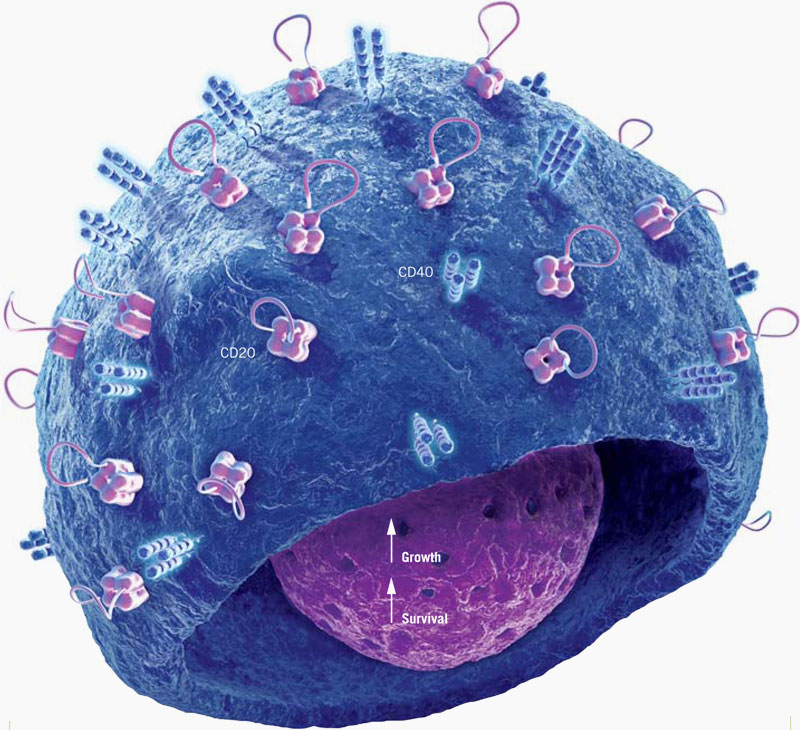
\includegraphics[height=50mm]{Cover/coverimage}
    \begin{tikzpicture}
      \clip (0,0)  circle (3cm) ;
      \node[anchor=center] at (-0.1,0) {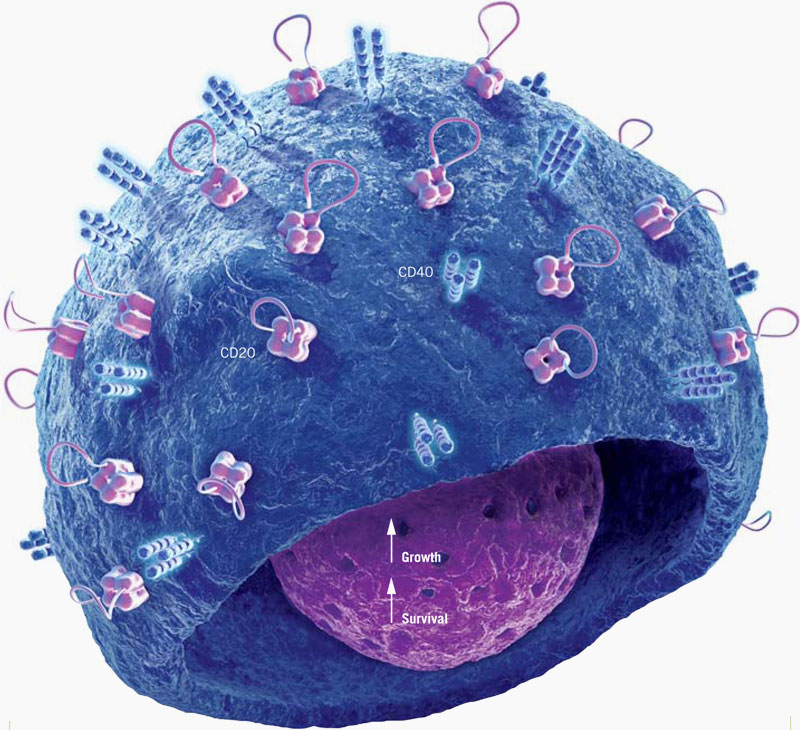
\includegraphics[height=6cm]{Cover/coverimage}};
      %adjust this coordinate to move image
    \end{tikzpicture}
  \end{center} % gráficos

  \vspace{5mm}
  \centering
  \LARGE \textbf{Memristors-based recurent modules for neural computing}
  \\ \vspace{15mm}
  \Large \textbf{Valentin BARBAZA} \\
  \vspace{12mm}
  \large Thesis to obtain the Master of Science Degree in
  \\ \vspace{2mm}
  \LARGE \textbf{Electrical and Computer Engineering}
  \\ \vspace{10mm}
  \large Supervisors: Dr. Diogo Caetano \\
  \large Dr. Ruxandra Barbulescu
  \\ \vspace{15mm}
  \Large \textbf{Examinatiom Committee}
  \\ \vspace{5mm}
  \large Chairperson: Prof. Lorem \\
  \large Supervisor: Prof. Lorem Ipsum\\
  \large Co-Supervisor: Prof. Lorem Ipsum \\
  \large Members of the Committe: Dr. Lorem Ipsum \\
  Prof. Lorem Ipsum

  \vspace{10mm}

  %\Large \textbf{\todaythesis\today} \\
  \Large \textbf{July/October 2023} \\
  \let\thepage\relax
\end{flushleft}
\pagebreak


\clearpage
% Since I am using double sided pages, the second page should be white.
% Remember that when delivering the dissertation, IST requires for the cover to appear twice.

\thispagestyle{empty}
\cleardoublepage

\setcounter{page}{1} \pagenumbering{roman}

\baselineskip 18pt % line spacing: -12pt for single spacing
%               -18pt for 1 1/2 spacing
%               -24pt for double spacingnts}
